\documentclass[a4paper,11pt]{article}
\usepackage[T1]{fontenc}
\usepackage[utf8]{inputenc}
\usepackage{lmodern}
\usepackage[francais]{babel}
\usepackage[ portrait, margin = 0.7 in]{geometry}
\usepackage{url}
\usepackage{amsmath}
\usepackage{graphicx}
\graphicspath{{~/Info/Projet/COROT}}
\usepackage{float}
\usepackage{subfig}
\numberwithin{equation}{section}


\begin{document}

\title{\LARGE \bf Détermination de la masse et du rayon d'une étoile par astérosismologie}
\author{MERCIER Wilfried - Observatoire de Paris}
\maketitle


\section{Astérosismologie}
\subsection{COROT}
COROT était un télescope de 27cm de diamètre permettant d'effectuer de la photométrie de précision. En opération de fin 2006 jusqu'à fin 2012, son principe était de 
mesurer de manière précise les faibles variations de luminosité de milliers d'étoiles et de détecter la présence d'exoplanètes par la méthode des transits\cite{COROT}.\newline
Les données que nous utiliserons par la suite proviennent de COROT et correspondent à la courbe de luminosité d'une étoile.
\subsection{Principe de l'astérosismologie}
Une étoile est une boule de gaz en équilibre hydrostatique qui à la suite de petites perturbations peut se mettre à osciller selon des modes de pression ou
de gravité\cite{modes}. Ces oscillations se manifestent par des variations de rayon (mesurées par spectroscopie) ou par des variations de luminosité.\newline
Dans ce qui suit, nous ne nous intéressons pas aux modes de gravité et aux méthodes par variation de rayon.\newline
L'étude des modes propres d'oscillation d'une étoile passe par la décomposition de son spectre en effectuant une analyse de Fourier. Les modes de pression étant régulièrement
espacés il est possible en étudiant le spectre en puissance de déterminer d'une part la fréquence correspondant à une puissance maximale notée $ \nu_{max} $ et d'autre part
la grande séparation, c'est-à-dire l'espacement en fréquence entre deux modes de pression consécutifs notée $ \Delta \nu$. 
À partir de ces deux données on peut déterminer la masse et le rayon de l'étoile via les formules\cite{eqs}

\begin{gather}
\label{sismo}
\frac{R_{*}}{R_{\odot}} = \frac{\nu_{max}}{\nu_{max\odot}} \left (\frac{\Delta \nu}{\Delta \nu_{\odot}} \right )^{-2} \left ( \frac{T_{eff,*}}{T_{eff\odot}} \right )^{0.5} \\
\label{sismo2}
\frac{M_{*}}{M_{\odot}} = \left ( \frac{\nu_{max}}{\nu_{max\odot}} \right )^{3} \left ( \frac{\Delta \nu}{\Delta \nu_{\odot}} \right )^{-4} \left ( \frac{T_eff,*}{T_eff\odot} \right )^{1.5}
\end{gather}

Où $R_{\odot} $, $M_{\odot}$, $\nu_{max\odot} = 3.15 \rm mHz$, $\Delta \nu_{\odot} = 134.9 \rm \mu Hz$ et $T_{eff\odot} = 5800 \rm K$  sont respectivement le rayon, la masse, la fréquence à la puissance maximale, la grande séparation et la température effective du Soleil. On associe alors à ces expressions les erreurs relatives suivantes

\begin{gather}
\label{erreur}
\left ( \frac{\delta R_*}{R_*} \right )^2 = \left ( \frac{\delta \nu_{max}}{\nu_{max}} \right )^2 + \left ( 2 \frac{\delta \Delta \nu}{\Delta \nu} \right )^2 + \left ( 0.5 
\frac{\delta T_{eff}}{T_{eff,*}} \right )^2 \\
\label{erreur2}
\left ( \frac{\delta M_*}{M_*} \right )^2 = \left (3 \frac{\delta \nu_{max}}{\nu_{max}} \right )^2 + \left ( 4 \frac{\delta \Delta \nu}{\Delta \nu} \right )^2 + \left ( 1.5 \frac{\delta T_{eff}}{T_{eff,*}} \right )^2
\end{gather}

\section{Description du projet}
On souhaite étudier la courbe de lumière de l'étoile HD52265 dont les données proviennent du satellite COROT afin de déterminer sa masse et son rayon grâce à l'astérosismologie.
On possède un signal d'une durée de 90j et 3h environs. On commence par construire le spectre en puissance de l'étoile en effectuant une analyse de Fourier de la courbe. Dans le cas d'un signal continu $s(t)$ sa transformée de Fourier s'écrit\cite{Fourier} (à un coefficient de normalisation près) comme

\begin{equation}
\tilde F(\nu) \propto \int_{-\infty}^{+\infty} s(t) e^{2 i \pi \nu t} dt
\end{equation}

Puisque l'on possède un signal discret on doit réécrire l'intégrale comme une somme de fréquences échantillonnées\cite{DFT} $\nu_k = k \delta \nu$ où $\delta \nu = 1/T$ est la résolution fréquentielle avec $T = 7786912 \rm s$ la durée d'observation. On peut alors décomposer notre transformée de Fourier en deux composantes, une partie réelle et une partie imaginaire données par

\begin{gather}
\tilde F_{reel}(\nu_k) = \frac{2}{N} \sum\limits_{i=1}^N s(i) \cos(2\pi\nu_k t(i))\\
\tilde F_{ima}(\nu_k) = \frac{2}{N} \sum\limits_{i=1}^N s(i) \sin(2\pi\nu_k t(i))
\end{gather}

Où $N = 243341$ est le nombre de points, $s(i)$ est le signal étudié et $t(i)$ est le temps correspondant. Les fréquences de Fourier varieront de 0 à $\nu_{max} = k_{m} 
\delta\nu$. Pour des raisons de temps de calcul on choisira $k_m = N\delta T \nu_c$, avec $\delta T = 32\rm s$ le temps entre deux observations et $\nu_c = 3\rm mHz$. On peut alors calculer pour chaque fréquence une puissance correspondante, c'est à dire le module carré de la transformée de Fourier

\begin{equation}
  P(\nu_k) = \tilde F_{reel}^2 (\nu_k) + F_{ima}^2(\nu_k)
\end{equation}

On obtient alors le spectre en puissance de l'étoile. Cette méthode ne peut fonctionner que si la résolution fréquentielle est très inférieur à la grande séparation. Il faudra donc vérifier cette condition avant d'étudier plus en détail le spectre. Une fois cela fait on sera en mesure de déterminer la fréquence à puissance maximale et la grande séparation puis à partir des équations \ref{sismo}, \ref{sismo2} déterminer la masse et le rayon de l'étoile.

\begin{figure}[H]
  \centering
  \subfloat[Vue large du spectre. Le pic central correspond \newline
  à la fréquence à la puissance maximale $\nu_{max}$]{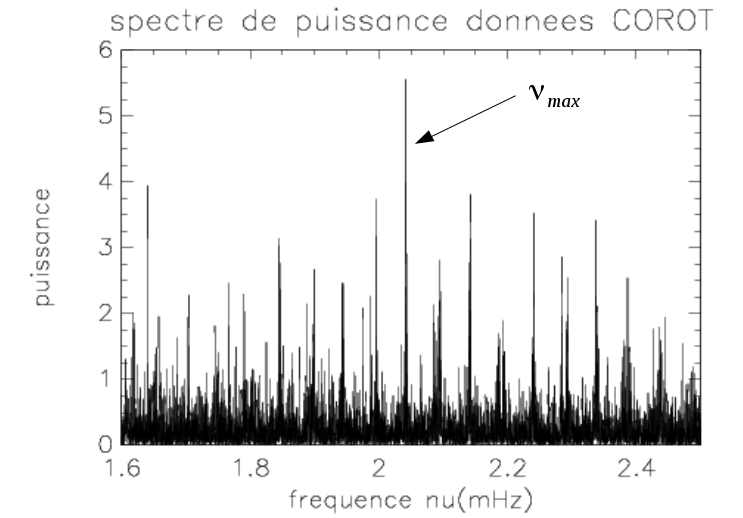
\includegraphics[width=0.49\linewidth]{puissance_52265_Mercier2_corrected_v2}}
  \subfloat[Vue agrandie de la partie droite du spectre. On remarque la grande séparation $\Delta \nu$ entre
  les deux pics principaux]{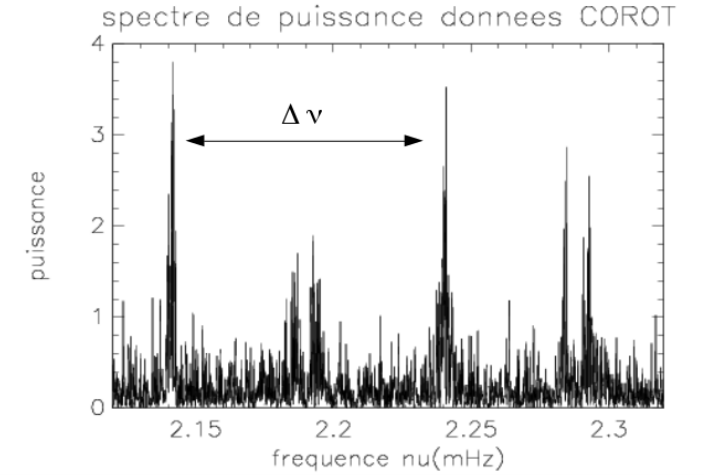
\includegraphics[width=0.49\linewidth]{puissance_52265_Mercier_corrected_v2}}
  \caption{Graphes du spectre en puissance de HD52265}
\end{figure}

\section{Résultats}
\subsection{Résultats personnels}
Le programme \textit{sismo\_Mercier.f90} (voir Annexe) retourne une résolution fréquentielle $\delta\nu \approx 0.1284 \rm \mu Hz$. En faisant l'hypothèse que HD52265 a une
grande séparation $\Delta \nu \sim \Delta \nu_{\odot}$, on a bien $\delta\nu \ll \Delta \nu$ et on peut utiliser le spectre en puissance retourné par l'analyse
de Fourier pour déterminer la grande séparation et la fréquence à la puissance maximale.\newline
Le spectre, ainsi que la fréquence à la puissance maximale et la grande séparation sont représentés en Figure 1. A partir du spectre et du programme \textit{plot\_puissance\_Mercier.pro} on trouve les valeurs suivantes pour la grande séparation et la fréquence à puissance maximale\newline

\begin{center}
$\Delta \nu = 99.035570 \rm \mu Hz$ \        \ $\nu_{max} = 2.0425540 \rm mHz$
\end{center}

On peut remarquer que l'hypothèse que $\Delta \nu \sim \Delta \nu_{\odot}$ était bien correcte. \newline
On peut alors utiliser \ref{sismo}, \ref{sismo2} avec $T_{eff,*} = (6100 \pm 60)\rm K$ pour en déduire la masse et le rayon. On obtient

\begin{center}
$M_{*} = 1.0123360188632631 \rm M_{\odot}$\   \ $R_{*} =  1.2338302244388120 \rm R_{\odot}$
\end{center}

\subsection{Résultats avec les données de Ballot et al.}
Ballot et al. avaient déterminés les valeurs de ces paramètres (avec leurs erreurs) de manière plus précise. Ils avaient trouvé $\Delta \nu = (98.3 \pm 0.1) \rm \mu Hz$ et
 $\nu_{max} = (2.09 \pm 0.02) \rm mHz$. 
À partir de ces paramètres, en utilisant les mêmes équations que précédemment ainsi que \ref{erreur} et \ref{erreur2} on trouve

\begin{center}
$M_{*} = (1.12 \pm 0.03) \rm M_{\odot}$\   \ $R_{*} =  (1.28\pm 0.01) \rm R_{\odot}$
\end{center}

\section{Conclusion}
L'analyse de Fourier sur les données de COROT a permis de déterminer la masse et le rayon de l'étoile à quelque chose comme 10\% près pour la masse et 5\% pour le rayon (par rapport aux données de Ballot et al.). L'étoile HD52265 est assez similaire au Soleil à la fois en terme de taille et de masse mais aussi en terme de température. D'après la loi de Stefan-Boltzmann ($L \propto R^2 T_{eff}^4$), en utilisant le rayon trouvé par Ballot et al., on en déduit une luminosité deux fois plus élevée que celle du Soleil. L'étoile se trouve donc encore sur sa séquence principale.\newline
La précision sur la masse et le rayon pourrait être accrue en utilisant des données sur une plus grande période de temps afin de réduire la résolution fréquentielle. De plus le temps de calcul de la transformée de Fourier est assez long (une dizaine de minutes pour ces données) et pourrait être grandement réduit en utilisant des algorithmes plus rapides comme des Transformées de Fourier Rapide (FFT). 

\newpage
\appendix
\section{Annexe : notice d'utilisation des programmes}
L'ensemble du code est séparé en trois programmes: le programme principal \textit{sismo\_Mercier.f90}, un module \textit{entree\_sortie\_Mercier.f90} qui lit les données de COROT puis écrit le spectre en puissance une fois calculé dans un fichier, et un module \textit{fourier\_Mercier.f90} se chargeant d'effectuer la transformée de Fourier discrète.\newline
\subsection{Étapes clés du programme principal \textit{sismo\_Mercier.f90}}

\begin{itemize}
  \item récupère les données en appelant la subroutine \textit{lecture\_corot} du module \textit{entree\_sortie\_Mercier.f90}
  \item calcule le nombre maximal de fréquences de Fourier $k_m$
  \item calcule la transformée de Fourier en faisant appel à la subroutine \textit{calcul\_fourier} de \textit{fourier\_Mercier.f90}
  \item écrit dans un fichier \textit{puissance\_52265\_Mercier.dat} le spectre en puissance en appelant la subroutine \textit{ecriture\_fourier} du module 
        \textit{entree\_sortie\_Mercier.f90}
\end{itemize}

\subsection{Module \textit{entree\_sortie\_Mercier.f90}}
Ce module contient deux subroutines \textit{lecture\_corot} et \textit{ecriture\_fourier}. \textit{lecture\_corot} est appelé dans le programme principal afin de lire les
données contenues dans le fichier \textit{hd52265\_corotdata.dat}.\newline
La subroutine \textit{ecriture\_fourier} se charge d'écrire dans le fichier \textit{puissance\_52265\_Mercier.dat} deux colonnes, la première contenant les fréquences de Fourier
et la seconde les puissances correspondantes.

\subsection{Module \textit{fourier\_Mercier.f90}}
Module contenant la subroutine \textit{calcul\_fourier} appelée depuis le programme principal pour calculer la partie réelle et la partie imaginaire de la transformée de Fourier pour l'ensemble des fréquences de Fourier. Cette subroutine renvoie les fréquences ainsi que les puissances dans le programme principal.

\bibliography{ref}
\bibliographystyle{ieeetr}
\end{document}
